\section{Theory behind the Faraday effect}
The \textit{Faradayeffect} refers to a megneto-optical phenomenon which can be explained in terms
of circular birefringence. The effect causes a rotation of the polarization direction with regards
to a applied magnetic field and its direction. It was discovered by \textit{faraday} in 1845 and
can be seen as the first experiment showing the interplay between light and electromagnetism. 
As already mentioned in the first part we can use the Maxwell equations to describe the magnetic
and electric field such that we can understand how the dielectricity of the material gives rise
to the phenomenon. For the experimental setup for seeing the faradayeffect you insert a medium,
which does not have to be optically active, between two polarizators. If we now fix the direction
of the magnetic field to be parallel to the direction of the incoming light we observe the 
already mentioned rotation.   
\subsection{Magneto-optic rotation}
As it turns out the first approximation the rotation angle of the polarization is proportional
to the Depth of the material $l$ and the magnetic field $B$:
\begin{equation}
    \alpha = V l B
\end{equation}
Where we introduced the Verdet-constant $V$. In the following we will derive this formula in order
to understand the physical nature of this constant \cite{staatsexamen}.
Lets assume without loss of generality a plane wave solution to the maxwell equation
with propagation in $z$-direction with speed v, 
entering the medium at $z=0$, being turned with the angle
$\alpha = \phi  z$:
\begin{align}
x &= F \cos{(\phi z)} \cos{\left ( \omega \left ( t - \frac{z}{v} \right )\right)} \\ 
y &= F \sin{(\phi z)} \cos{\left ( \omega \left ( t - \frac{z}{v} \right )\right)}
\end{align}
if we now apply $\cos(\beta) = (e^{i\beta} + e^{-i\beta})/2$ 
(analogous $\sin(\beta) = (e^{i\beta} - e^{-i\beta})/2i$ )
and rename $\tau := (t-\frac{z}{v})$:
\begin{align}
x &= \frac{F}{4} \left (e ^{i\phi z} + e ^{-i\phi z} \right )
\left (e ^{i\omega \tau} + e ^{-i\omega \tau} \right ) \\ 
&= \frac{F}{2} \left ( \cos{(\phi z + \omega \tau)} + \cos{(\omega \tau -  \phi z )} \right ) \\
\Rightarrow y &= \frac{F}{2} \left ( \sin{(\phi z + \omega \tau)} - \sin{(\omega \tau -  \phi z )} \right )
\end{align}
which in particular shows how the linear polarized wave consists of two circular, reverse polarized
waves with relatives speeds:
\begin{align}
\frac{\omega}{v_+} &= \frac{\omega}{v} - \phi \label{eq:v+}\\ 
\frac{\omega}{v_-} &= \frac{\omega}{v} + \phi \label{eq:v-}
\end{align}
Subtracting these two equations yields
\begin{equation}
2\phi = \omega \left (\frac{1}{v_-} - \frac{1}{v_+} \right)
\end{equation}
which we can insert into the definition of $\alpha$ and the refraction index $n = c/v$:
\begin{align}
\alpha = \phi l &= \frac{\omega l}{2} \left (\frac{1}{v_-} - \frac{1}{v_+} \right) \\ 
 &= \frac{\omega l}{2c} \left (n_- - n_+ \right)
\end{align}
From equation \eqref{eq:v+} and \eqref{eq:v-} we get (implying for tiny $\phi$ in the last step):
\begin{equation}
v_{+/-} = \frac{\omega}{\frac{\omega}{v} \mp \phi} = \frac{v}{1 \mp \frac{\phi v}{\omega}} 
= v \left ( 1 \pm \frac{\phi v}{\omega}+ \left (\frac{\phi v}{\omega} \right)^2
\pm \left (\frac{\phi v}{\omega} \right)^3 + \left (\frac{\phi v}{\omega} \right)^4+ \cdots \right)
\approx v \left  (1 \pm \frac{\phi v}{\omega} \right )
\end{equation}
Using the semiclassical Bohrmodel we can understand the behavior of the electrons in 
first approximation with the Larmorfrequency:
\begin{equation}
\omega_L = \frac{-e B}{2 m c}
\end{equation}
Since the dynamics of the electrons is fundamentally connected to the dispersion of the material,
we can use this frequency to connect the Rotation of the polarization with the dynamical behavior 
of the electrons of the medium. If we go into a coordinatesystem which is rotating with $\omega_L$,
the electrons have their original frequency (predicted by the Bohr model), hence the electromagnetic
wave is shifted by this frequency with regards to the original coordinate system. Thus we get:
\begin{equation}
\alpha = \frac{\omega l}{2c} \left (n_{\omega + \omega_L} - n_{\omega - \omega_L}\right )  
\end{equation}
The refraction index in dependence of the frequency is given by the dispersion relation, which is 
dependent on the medium. For tiny frequencies we can taylor: 
\begin{equation}
n(\omega + \omega_L) \approx n(\omega) \pm \omega_L \frac{\partial n}{\partial \omega}
\end{equation}
and now we can write in this in terms of $\omega \frac{n}{w} = -\lambda \frac{n}{\lambda}$:
\begin{equation}
\alpha = \frac{\omega_L l \lambda}{c} \frac{\partial n}{\partial \lambda} = 
\frac{e l B \lambda}{2m c^2} \frac{\partial n}{\partial \lambda} \quad \text{Formula of Bequerel}
\end{equation}


\subsection{Experimental setup}
The setup of our experiment is as following: We have a coil as an inductor in which the light
surpasses a flintglass, which is inside of the coil (see figure~\ref{fig:faraday_setup}). The
coil is being cooled by a cooling unit. The water is supplied by an external  water feed pipe
and flowing of with a drainage. The light is emitted by a sodium light. After it goes through
the halfshade polarizer, then the coil and again through a polarizer when we can finally 
observe it with the eyelet. We can rotate the second polarizer 
to analyze the polarization direction of the incoming light and change the current flowing through
the coil.

\begin{figure}
    \begin{centering}
        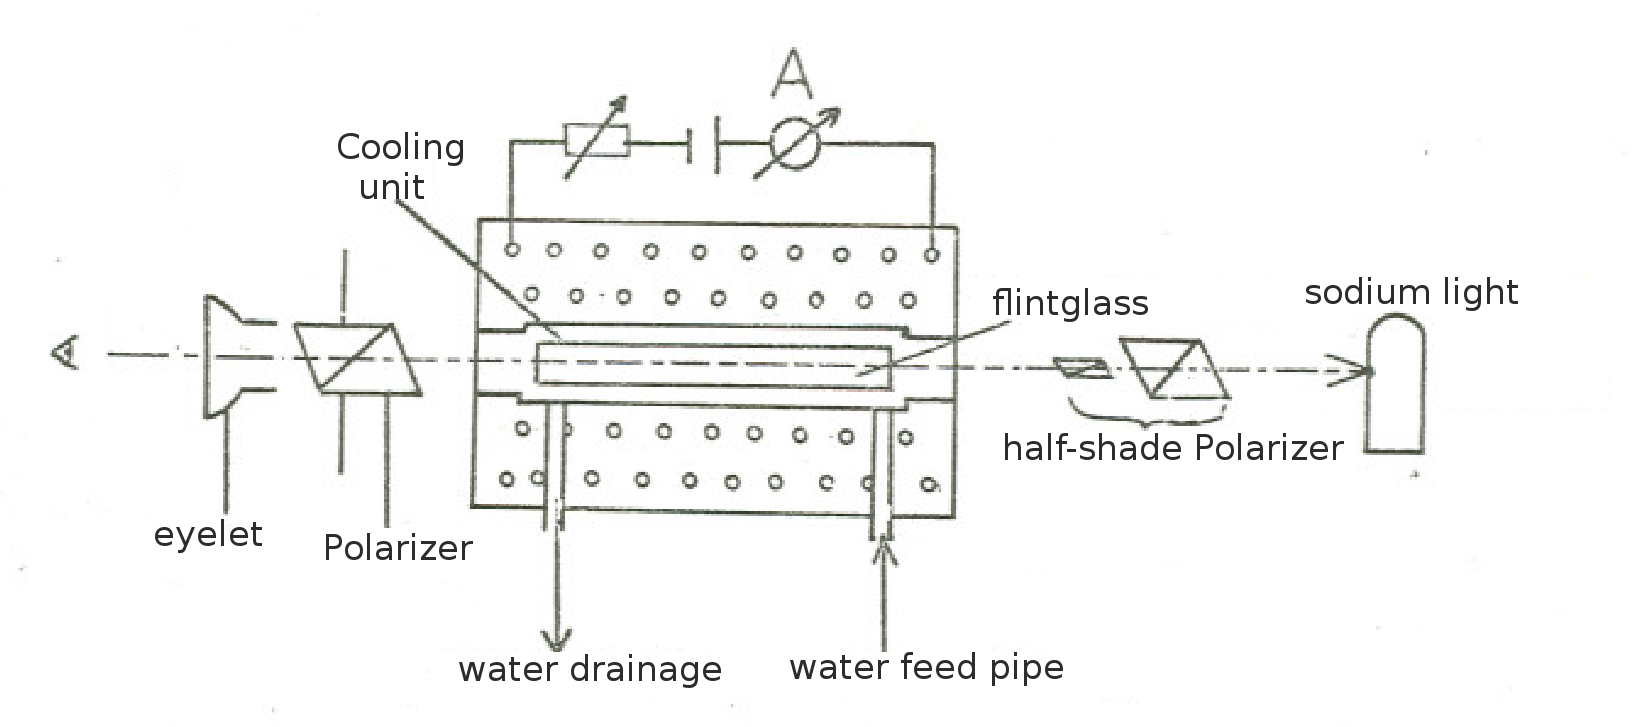
\includegraphics[width=18cm]{figures/faraday_setup2}
        \caption{Experimental setup (figure from \cite{staatsexamen}).}
        \label{fig:faraday_setup}
    \end{centering}
\end{figure}

\subsection{Half shade polarizer}
The halfshade polarizer functions as following. We use a Nicol prism, which was invented in
1828 by William Nicol. Its essentially a rhombohedral crystal of iceland spar with a 69 degree cut with
respect to the optical axis of the crystal, another diagonal cut only to be attached to each
other again. The two Nicols in the device are used differently: The large Nicol polarizes the
incoming light of the sodium lamp while the tiny Nicol rotates the polarization plane of 
a part of the light with an angle $\epsilon$. This is the reason why in the end we see different
areas with different degree of intensity in the eyelet (see figure~\ref{fig:halfshadepolarizer}).
Since it is more convenient for the eye to recognize the case with equal intensity than to
distinguish the case with different areas, we will use it for analyzing the rotation angle.
If we now turn on the magnetic field $B$ we observe the rotation of the incoming light, which
now can be tracked down by adjusting the analyzer to regain the state with equal intensity.
\begin{figure}
    \begin{centering}
        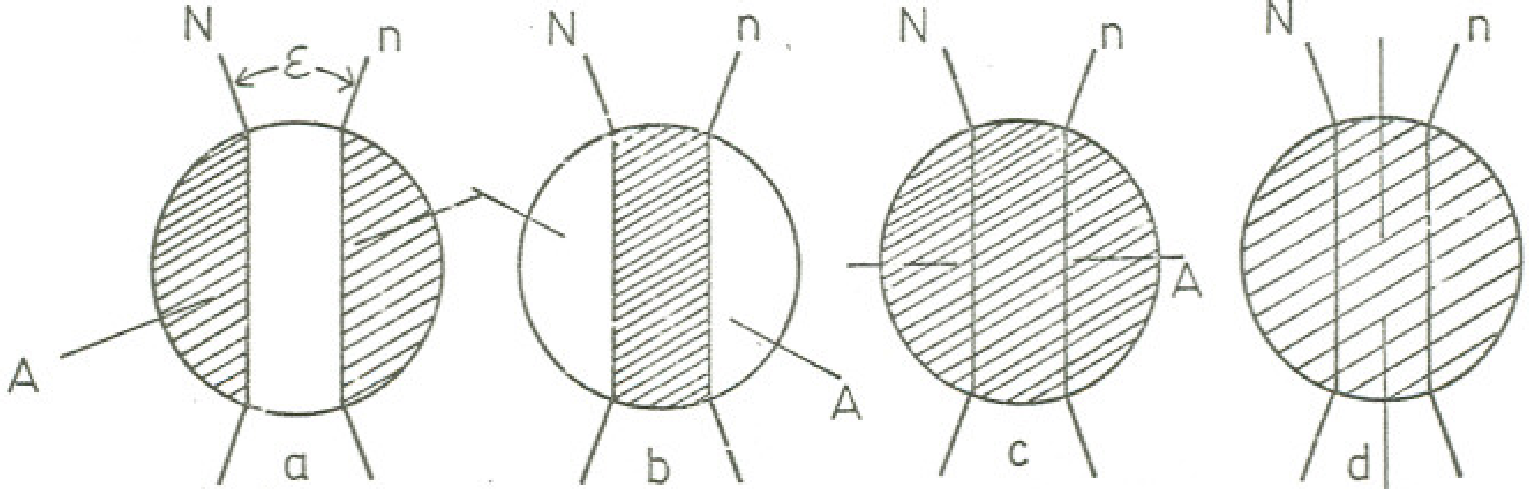
\includegraphics[width=14cm]{figures/halfshadepolarizer}
        \caption{Half shade polarizer (figure from \cite{staatsexamen}) where we used the
            abbreviations: \\
            $N$ = polarization direction of the large Nicol\\
            $n$ = polarization direction of the tiny Nicol\\
            $A$ = polarization direction of the second polarizer\\
            In the experiment we use the configuration c), since it is most convenient
            for the eye to recognize and thus can resample the best precision.
            }
        \label{fig:halfshadepolarizer}
    \end{centering}
\end{figure}
\subsection{Magnetic field inside of the coil}
We start with the law of Biot-Savart of a electric flow $I$ along the path $C$ which generates
a magnetic field $B$ at position $r$:
\begin{equation}
    \vec{B} = \frac{\mu_0}{4\pi} \int_{C} \frac{I d\vec{l} \times \vec{r}}{|\vec{r}|^3} 
\end{equation}
which can be rewritten, if we use the absolute value instead of vectors and the Radius $r$ of the
coil with the horizontal position $x$:
\begin{equation}
    dB = \frac{\mu_0}{4\pi} \frac{N \cdot I dl}{r^2 + x^2} 
\end{equation}

We only need the fraction of the x-direction. Let now $\theta$ be the angle betwen the $y,z$ 
direction and the $x-$axis using $\sqrt{{l'}^2 + x^2} \cos(\theta) = {l'}$:
\begin{align}
    \Rightarrow dB_x &= dB \cos\theta = dB \left (\frac{{l'}}{\sqrt{{l'}^2 + x^2}} \right) = 
    \frac{\mu_0}{4\pi} \frac{N\cdot I  \cdot {l'} \cdot dl}{\sqrt{\left ({l'}^2 + x^2 \right )^3}} \\
    B_x &= \frac{\mu_0}{4\pi} \frac{N\cdot I  \cdot {l'}}{\sqrt{\left ({l'}^2 + x^2 \right )^3}} \int_C dl 
  = \frac{\mu_0}{4\pi} \frac{N\cdot I  \cdot {l'}}{\sqrt{\left ({l'}^2 + x^2 \right )^3}} \left (2\pi {l'} \right )
  =  \frac{\mu_0}{2} \frac{N\cdot I  \cdot {l'}^2}{\sqrt{\left ({l'}^2 + x^2 \right )^3}} 
\end{align}
We now define the following quantities, see figure~\ref{fig:integral}: 
\begin{itemize}
\setlength\itemsep{0.0mm}
    \item[$x,y,z$] \ldots respective lengths in directions of the coordinate system 
    \item[$l$]     \ldots length of the flint glass, in our case $l=150$mm.
    \item[$L$]     \ldots length of the Coil, in our case $L=175$mm.
    \item[$2x_1$]  \ldots inner diameter of the coil $2x_1=20$mm
    \item[$2x_2$]  \ldots outer diameter of the coil $2x_2=150$mm 
\end{itemize}

\begin{figure}
    \begin{centering}
        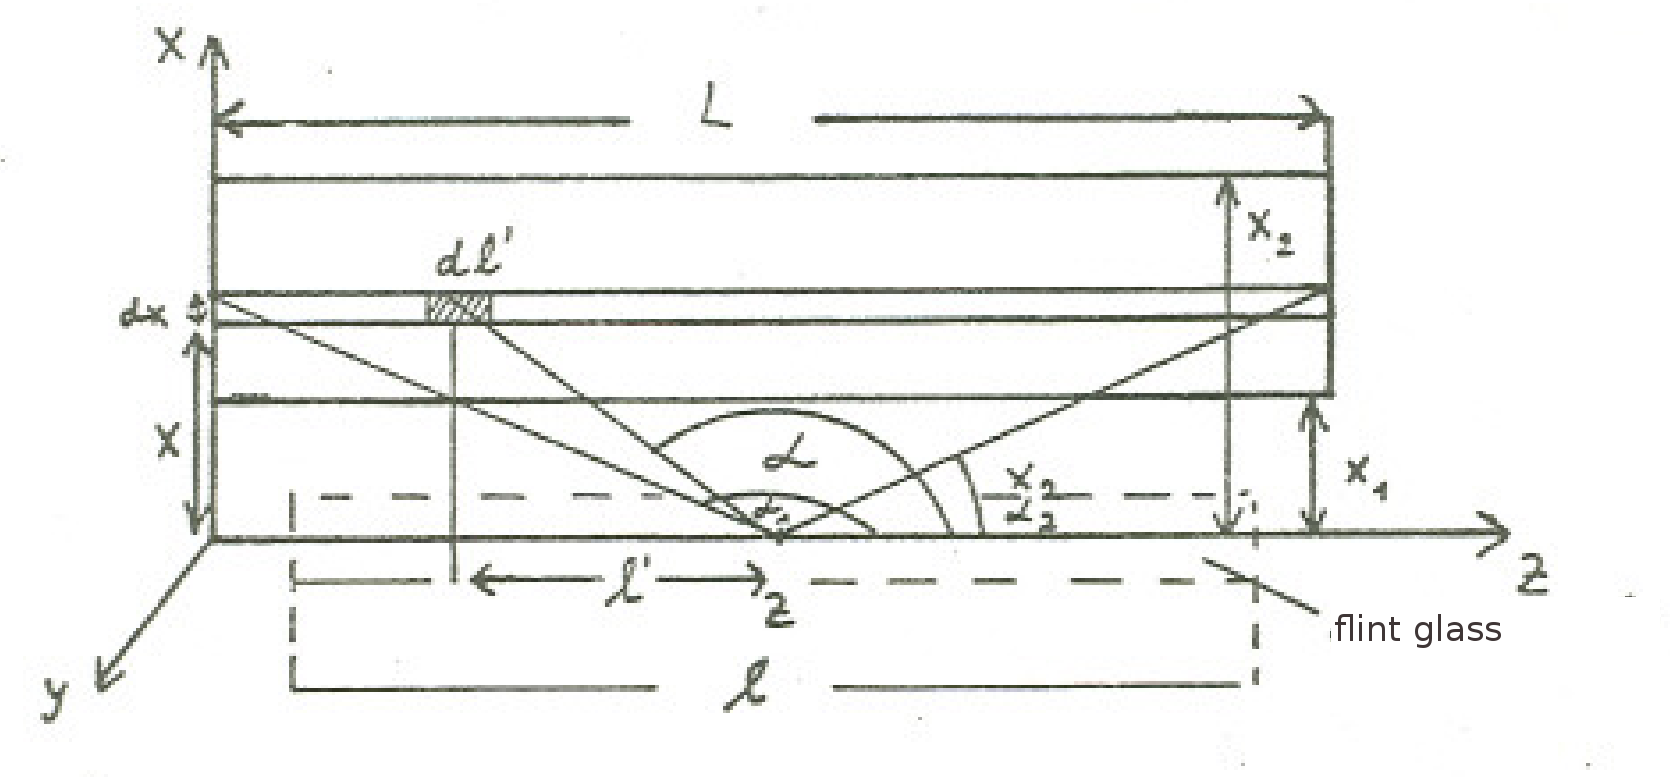
\includegraphics[width=14cm]{figures/integral}
\caption{Sketch from the variables (figure from \cite{staatsexamen}) which we will use
            for calculating the integral. 
            }
        \label{fig:integral}
    \end{centering}
\end{figure}
Now we look at the surface element which is sketched in figure~\ref{fig:integral},
arriving at:
\begin{equation}
 \delta B_x =  \frac{\mu_0}{2} \frac{N \cdot \delta I  \cdot R^2}{\sqrt{\left (R^2 + x^2 \right )^3}} ,
 \quad \delta I = \frac{ I \cdot dx \cdot dl'}{L(x_2 - x_1)}
\end{equation}
Now we get by inserting the $\delta I$ into the magnetic field and integrating over
the whole $x$-axis (which we will denote for simplicity by $H$ with $B = \mu H$):
\begin{align}
    H &= \underbrace{ \frac{ N\cdot I}{2 L (x_2 - x_1)} }_{:=\beta}
    \int^{L-z}_{-z} \int^{x_1}_{x_2} \frac{x^2}{(x^2 + l'^2)^{3/2}} dx dl'\\
\end{align}
Now and in what follows we can use the integrals:
\begin{align}
    \int \frac{a^2 dy}{(a^2 + y^2)^{3/2}}&=  \frac{y}{\sqrt{a^2 + y^2}} \\
    \int \frac{dy}{(a^2 + y^2)^{1/2}} &=  \log{\left [ y + \sqrt{a^2 + y^2} \right]}\\
    \int \frac{y dy}{\sqrt{y^2 + a^2}} &= \sqrt{y^2 + a^2} \\
    \int \sqrt{y^2 + a^2} dy &= \frac{1}{2} \left(
    y \sqrt{ y^2 + a^2} + a^2 \log \left [ y + \sqrt{y^2 + a^2} \right ] 
        \right )
\end{align}
which is easy to see if you differentiate the right side respectively. From this follows:
\begin{align}
    H &= \beta  \int^{x_2}_{x_1} \left (  \frac{L - z}{\sqrt{x^2 + (L-z)^2}} +
      \frac{z}{\sqrt{x^2 + z^2}}    \right ) dx  \\
  &= \beta  \left (
  (L-z) \log{\left [ \frac{x_2 + \sqrt{(L-z)^2 + x_2^2}} { x_1 + \sqrt{(L-z)^2 + x_1^2}} \right]}
  +z \log{\left [ \frac{x_2 + \sqrt{z^2 + x_2^2}} { x_1 + \sqrt{z^2 + x_1^2}} \right]}
  \right)
\end{align}
which is in the middle of the coil with $z = L/2$:
\begin{equation}
    H(z = L/2) = \beta \cdot L \cdot
    \log{\left [ \frac{x_2 + \sqrt{(\frac{L}{2})^2+ x_2^2}} { x_1 + \sqrt{(\frac{L}{2})^2 + x_1^2}} \right]}
\end{equation}
which is with our specifications of the experimental setup:
\begin{align}
    H( z = 87.5 \mathrm{mm}) &=   \left [ 1.84 \pm 0.02\right ] 10^5\quad  \mathrm{A/m} \\
         &=  \left [ 2305 \pm 26\right ] \quad \mathrm{Oe}
\end{align}
If we would have used $H= N \cdot I / L$ we got:
\begin{align}
    H( z = 87.5 \mathrm{mm}) &=   \left [ 2.057 \pm 0.024\right ] 10^5\quad  \mathrm{A/m} \\
         &=  \left [ 2585.1\pm29.8\right ] \quad \mathrm{Oe}
\end{align}
Which is far away from our obtained result but good for estimating the magnetic field fast.
\subsection{Integral of the rotation angle}
Now we pursue to calculate the angle $\alpha$ by $d\alpha = V H(z) dz$,
following from the magnetic field we just calculated but not only integrating over $x$, but
also over $z$:
\begin{align}
    \alpha &= V\ \cdot\beta  \int^{z=\frac{L+l}{2}}_{z=\frac{L-l}{2}} \int^{x_1}_{x_1}
    \left (  \frac{L - z}{\sqrt{x^2 + (L-z)^2}} +
      \frac{z}{\sqrt{x^2 + z^2}}    \right ) dx dz \\
  &=  2 \cdot V\ \cdot\beta  \int^{x_1}_{x_1}
    \left (  
        \sqrt{x^2 + \left (\frac{L+z}{2}\right )^2} -\sqrt{x^2 + \left (\frac{L-z}{2}\right )^2}
        \right ) dx  
    \end{align}
Which then results into:
\begin{equation}\label{e:barwq}\begin{split}
=   V\beta \bigl [
     x_2 \left (\sqrt{ x_2^2 + \frac{(L+l)}{4}^2}- \sqrt{ x_2^2 + \frac{(L-l)}{4}^2}\right ) 
     -x_1 \left (\sqrt{ x_1^2 + \frac{(L+l)}{4}^2}- \sqrt{ x_1^2 + \frac{(L-l)}{4}^2}\right )  \\
    +\left (
    \frac{(L+l)}{4}^2 \log{
        \left [ \frac{x_2 + \sqrt{\frac{(L+l)}{4}^2  + x_2^2}} { x_1 + \sqrt{\frac{(L+z)}{4}^2 + x_1^2}} \right]}
- \frac{(L-l)}{4}^2 \log{
        \left [ \frac{x_2 + \sqrt{\frac{(L-l)}{4}^2  + x_2^2}} { x_1 + \sqrt{\frac{(L-z)}{4}^2 + x_1^2}} \right]}
  \right)
    \bigr ]
\end{split}\end{equation}
When we now plug in the specifications of our setup we get:
\begin{align}
    \alpha = V \cdot I \cdot \left (2587.5\pm16.4 \right )
\end{align}


